% Automatically generated figure inventory for task3.

\begin{figure}[H]
\centering
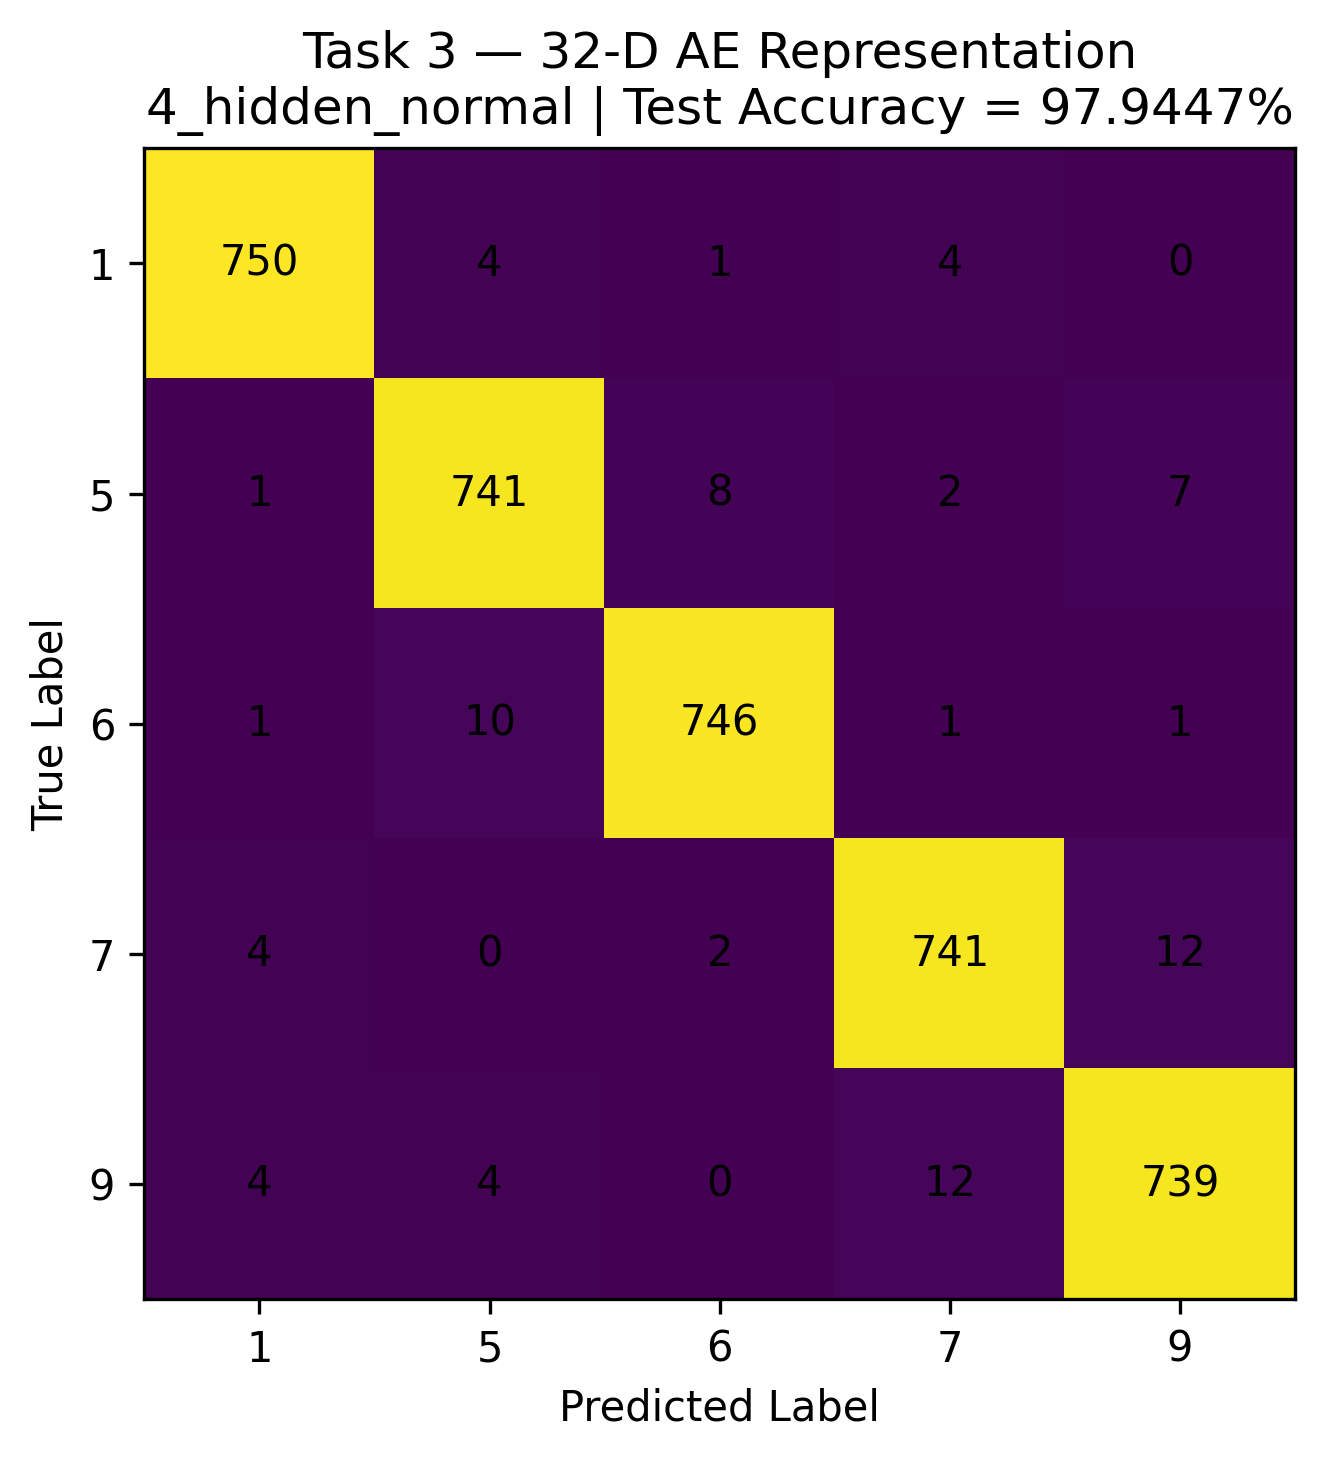
\includegraphics[width=0.88\linewidth,height=0.34\textheight,keepaspectratio]{figures/task3/cnf_matrics_img/confusion_matrix_32.png}
\caption{Confusion matrix: confusion matrix for 32 neurons bottleneck.}
\label{fig:task3_1}
\end{figure}

\begin{figure}[H]
\centering
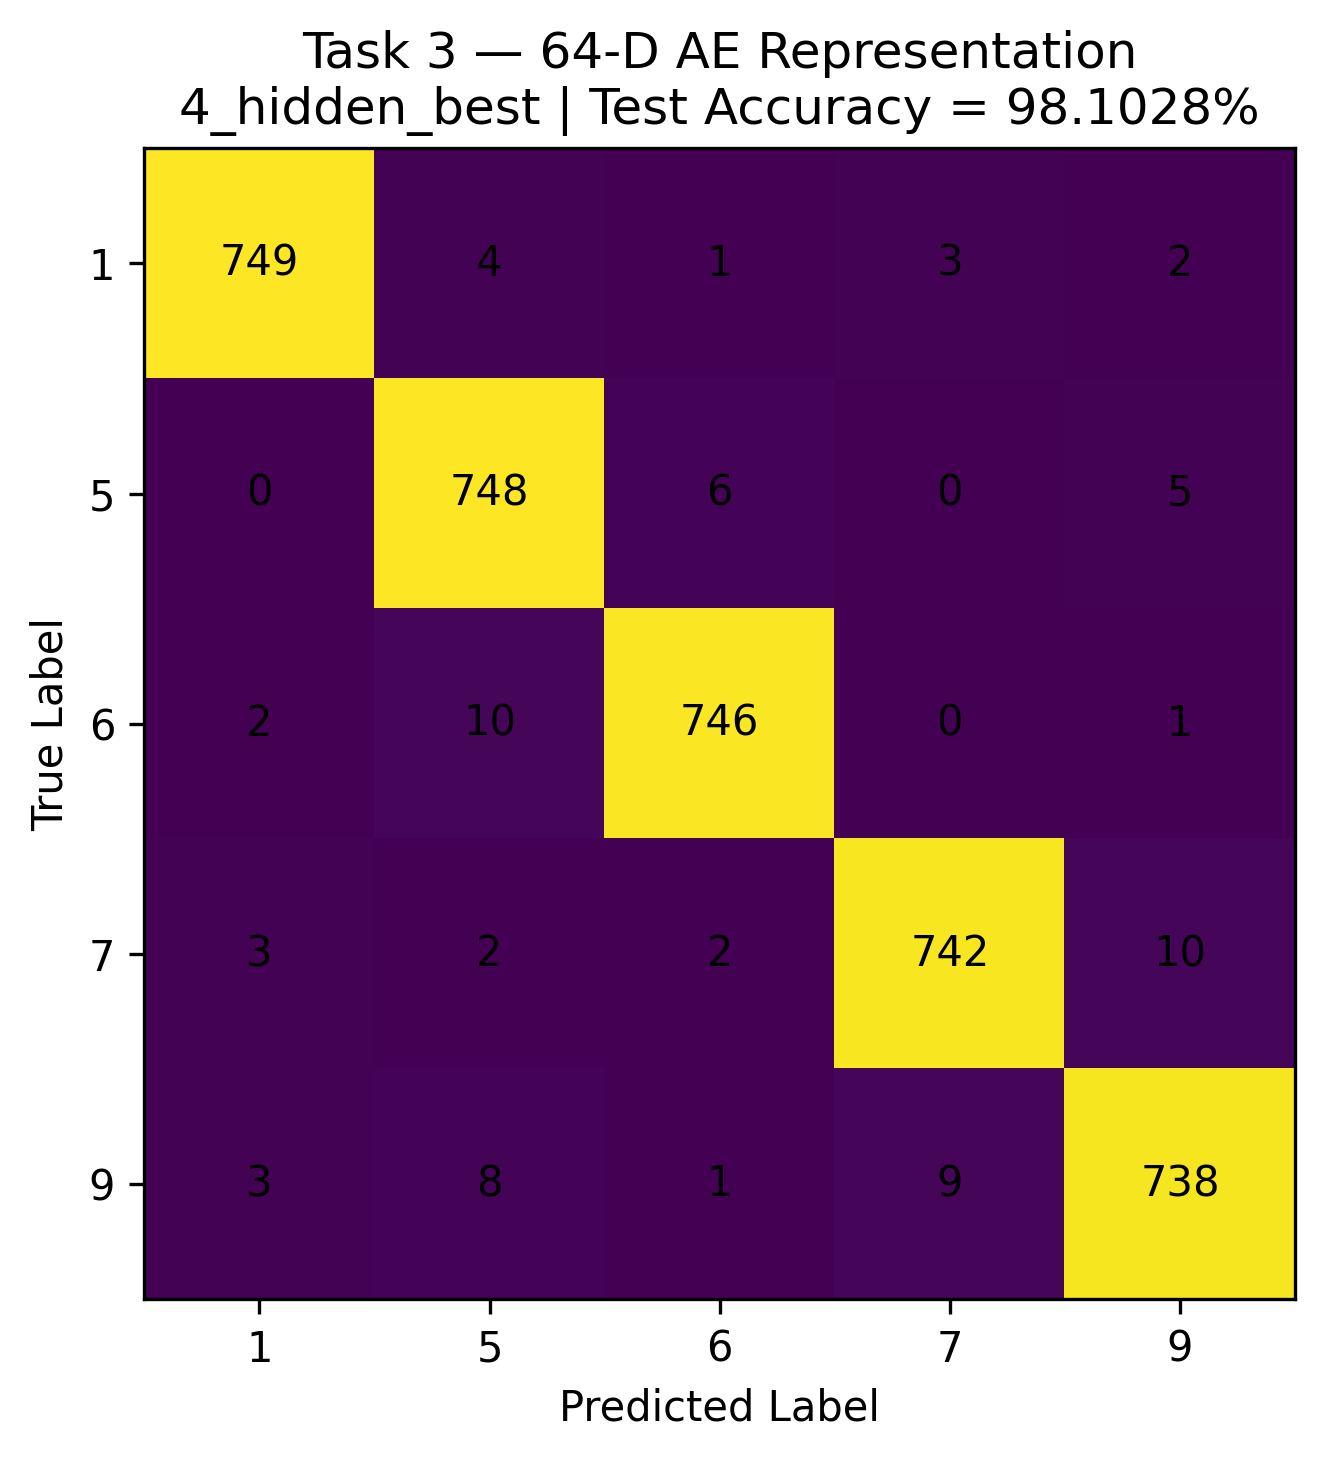
\includegraphics[width=0.88\linewidth,height=0.34\textheight,keepaspectratio]{figures/task3/cnf_matrics_img/confusion_matrix_64.png}
\caption{Confusion matrix: confusion matrix for 64 neurons bottleneck.}
\label{fig:task3_2}
\end{figure}

\begin{figure}[H]
\centering
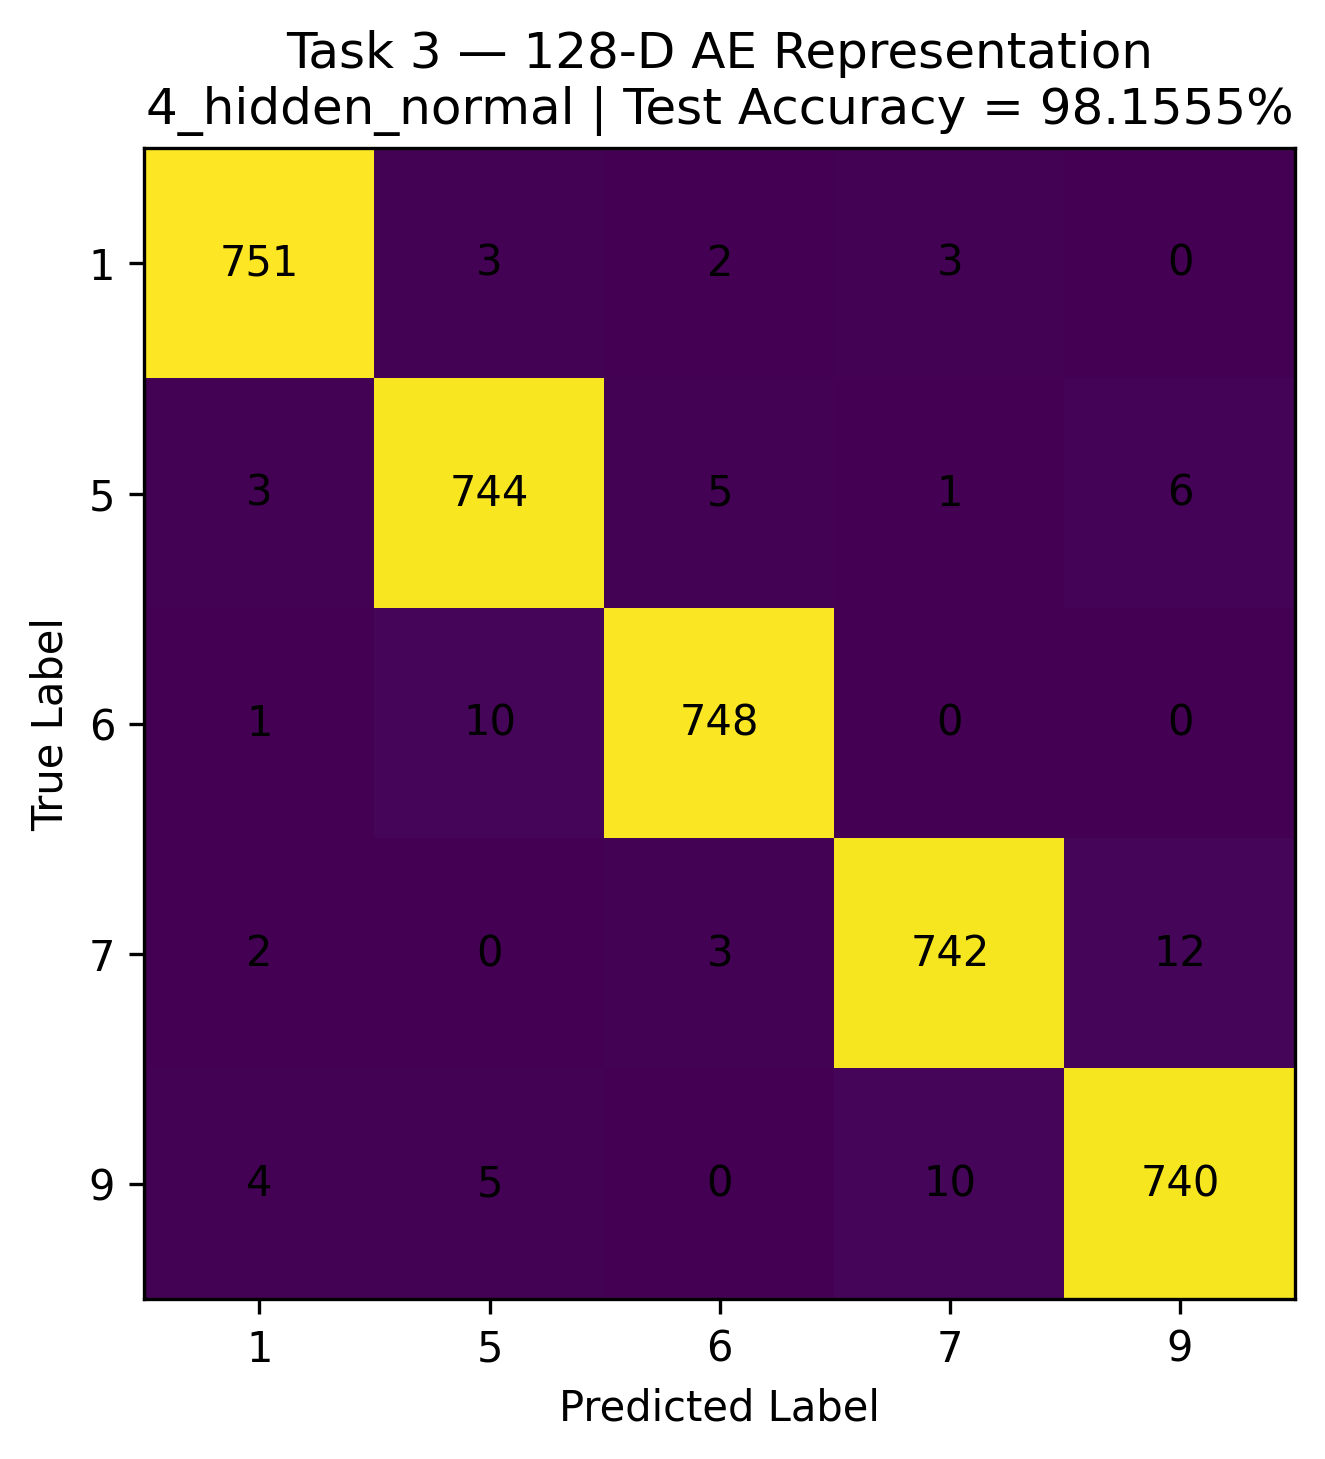
\includegraphics[width=0.88\linewidth,height=0.34\textheight,keepaspectratio]{figures/task3/cnf_matrics_img/confusion_matrix_128.png}
\caption{Confusion matrix: confusion matrix for 128 neurons bottleneck.}
\label{fig:task3_3}
\end{figure}

\begin{figure}[H]
\centering
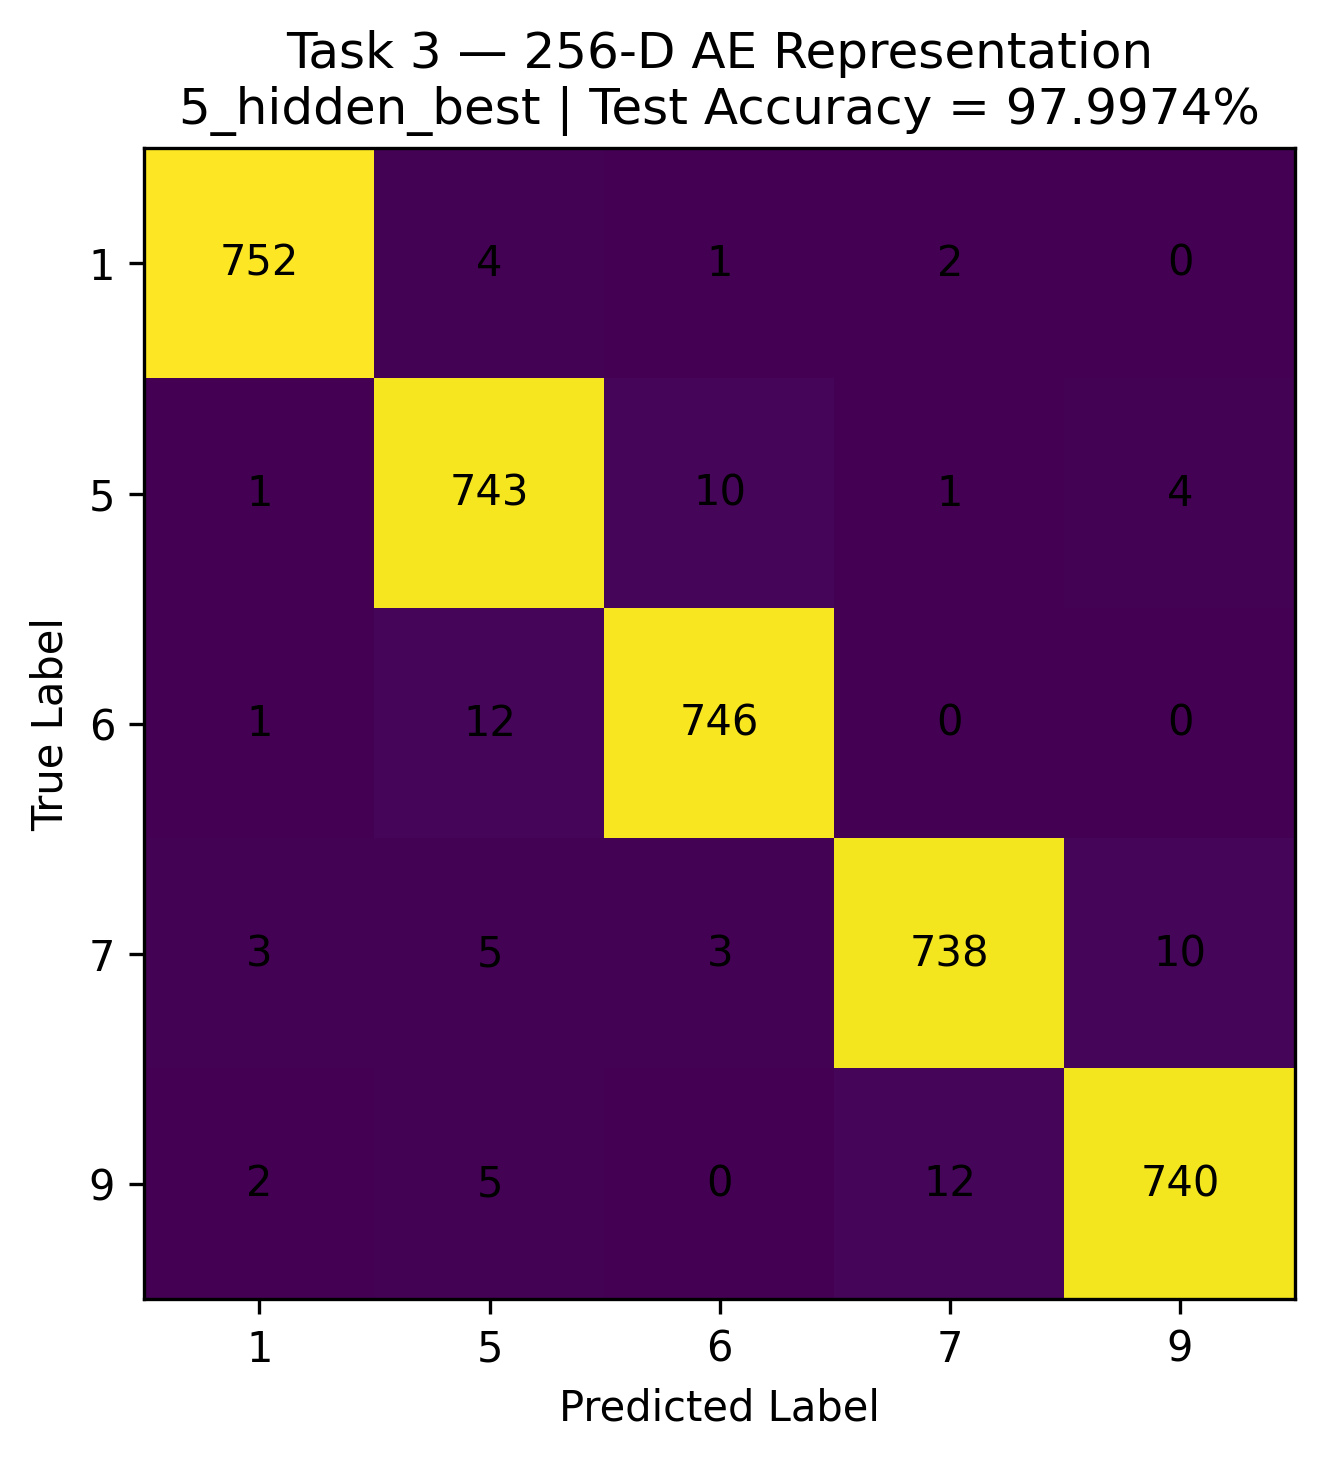
\includegraphics[width=0.88\linewidth,height=0.34\textheight,keepaspectratio]{figures/task3/cnf_matrics_img/confusion_matrix_256.png}
\caption{Confusion matrix: confusion matrix for 256 neurons bottleneck.}
\label{fig:task3_4}
\end{figure}
